\subsection{RQ3: What type of testing and deployment practices are used?}
\label{RQ3}
Testing is an important process in improving the quality of the software product. The purpose of this process is to find errors, which might occur during specification, design and code generation. Here we report the following results next:
\begin{itemize}
\item Software Testing Practices (Q 14)
\item Level of Automated Testing (Q 15)
\item Tools Used in Testing and QA (Q 16)
\item Continuous Deployment tools (Q 17)
\item Version Control (Q 18)
\end{itemize}

\subsubsection{Software Testing Practices}
According to \cref{fig:testing}, several number of testing practices are used during software development. The results show most of the organizations carried out unit testing(24\%), functional testing(20\%), user acceptance testing(17\%), GUI testing(14\%) etc.
\begin{figure}[]
\centering
  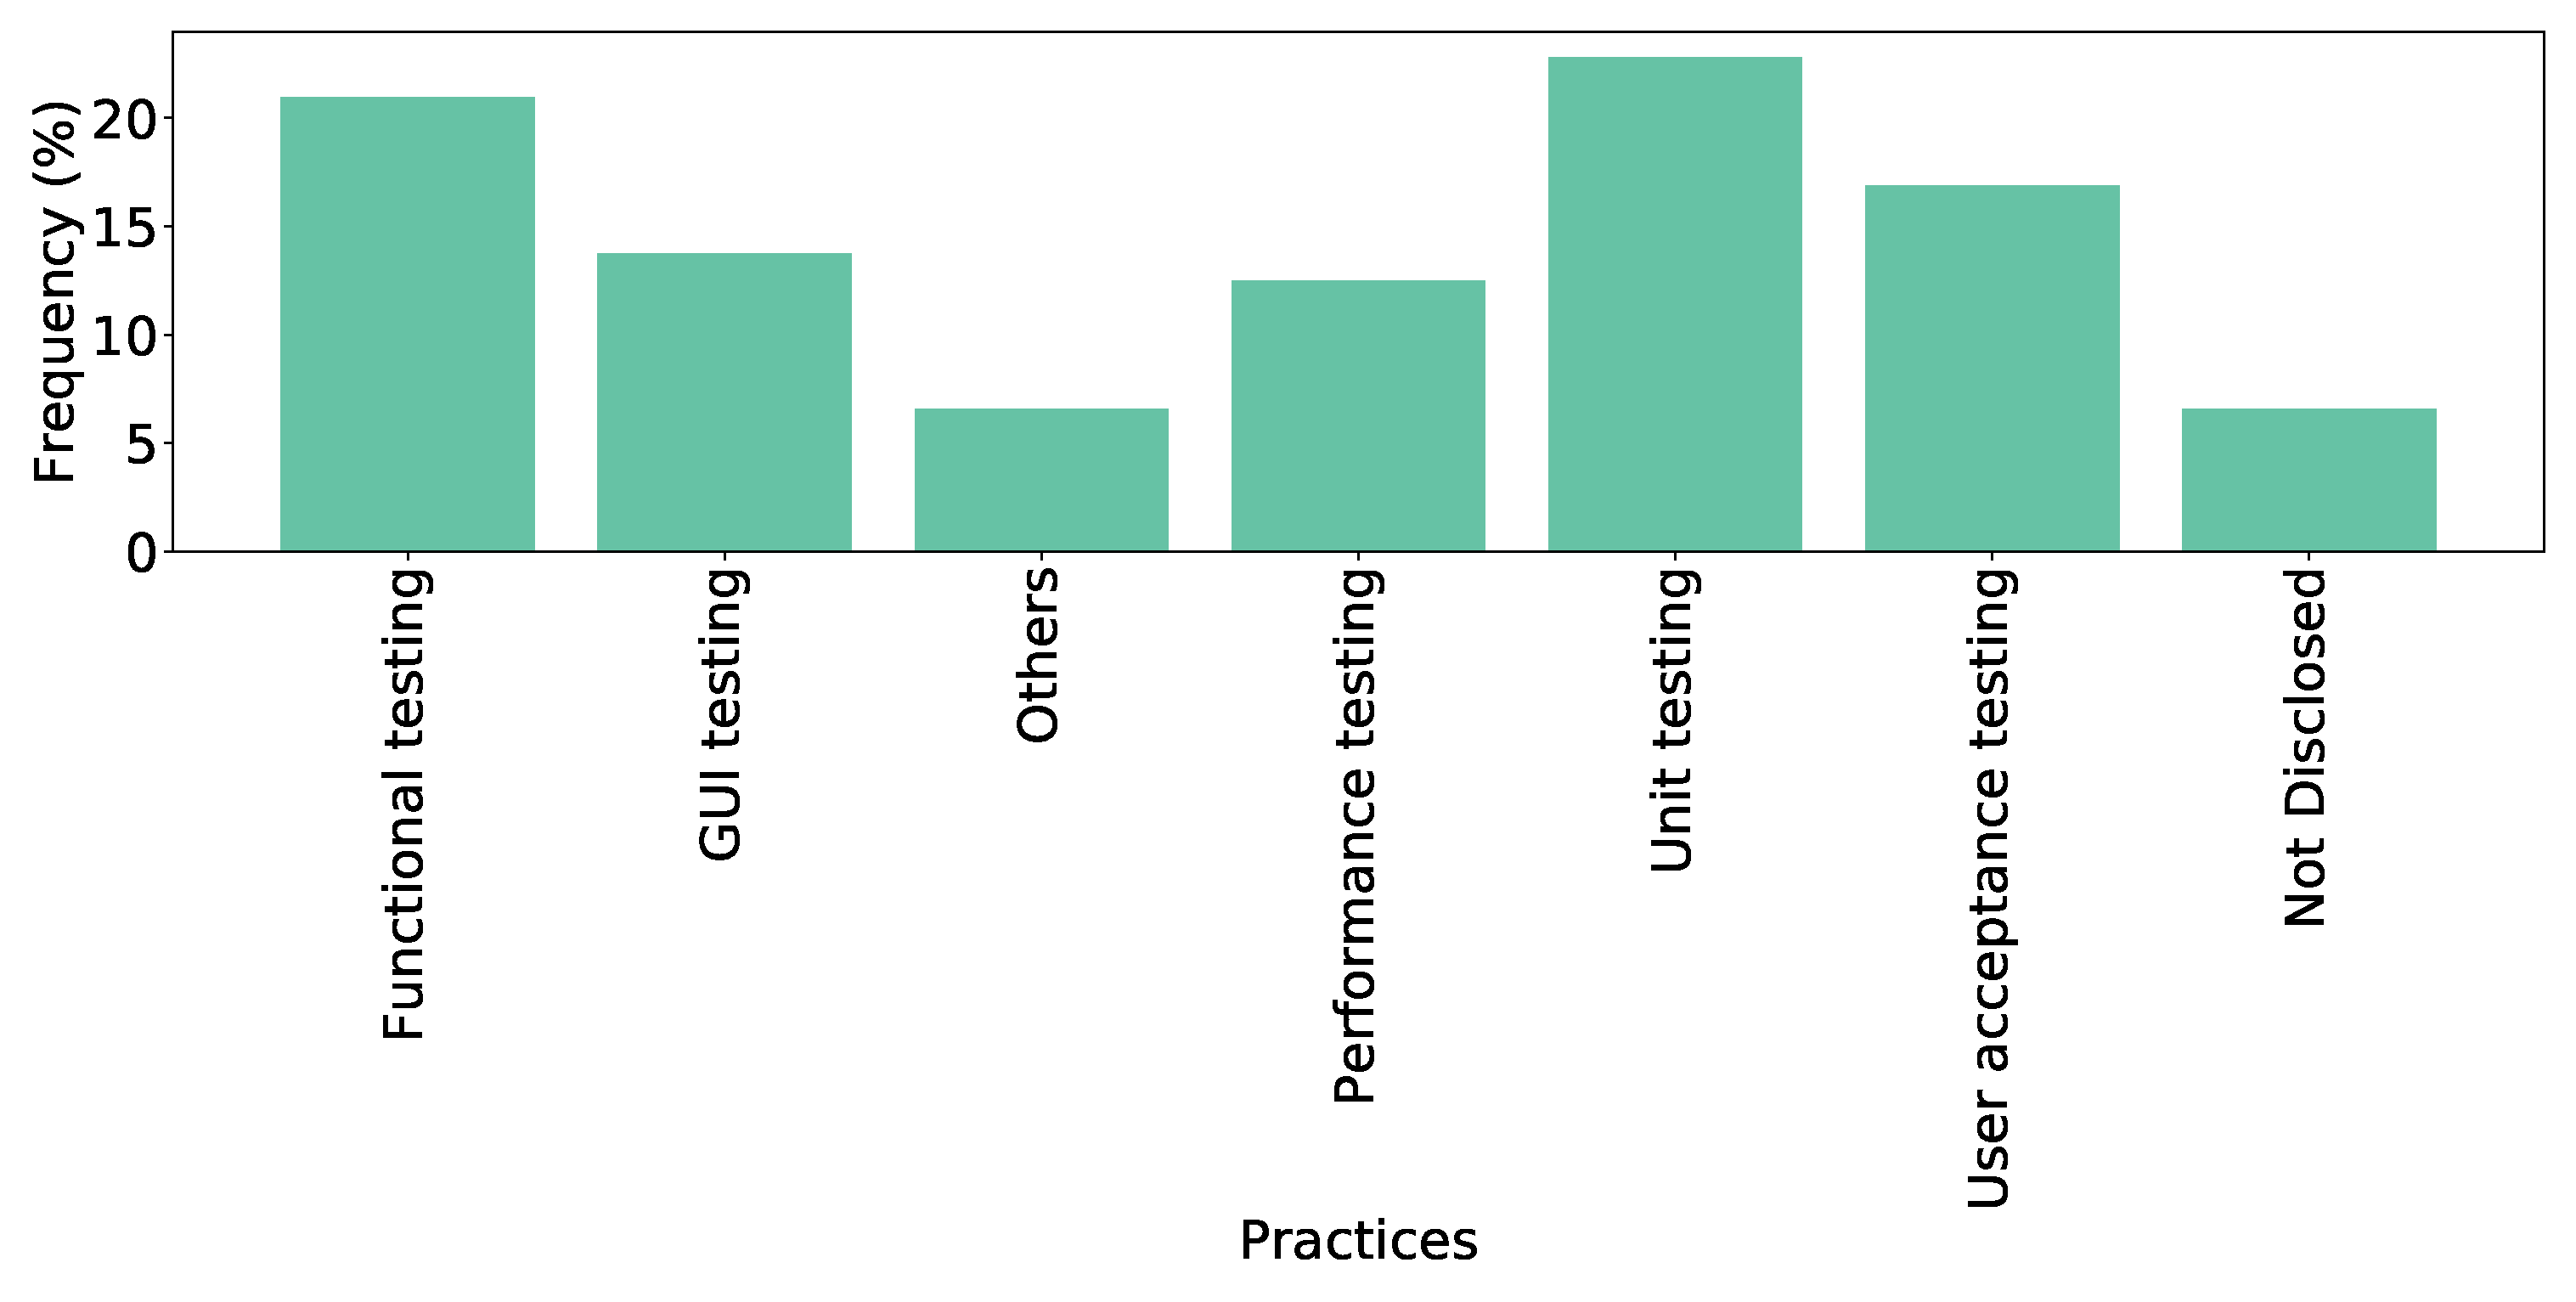
\includegraphics[width=0.8\textwidth]{Figures/Respondents_testing_practices}
  \caption{Testing Practices}
  \label{fig:testing}
\end{figure}

\subsubsection{Level of Automated Testing}
Question 15 asked about the level of automated testing. The responses were gathered using the Likert scale. This denotes that different respondents have very different practices in this context, i.e., some heavily practice automated testing, while others favor manual testing. Results are shown in \cref{fig:autoTest}.
\begin{figure}[]
\centering
  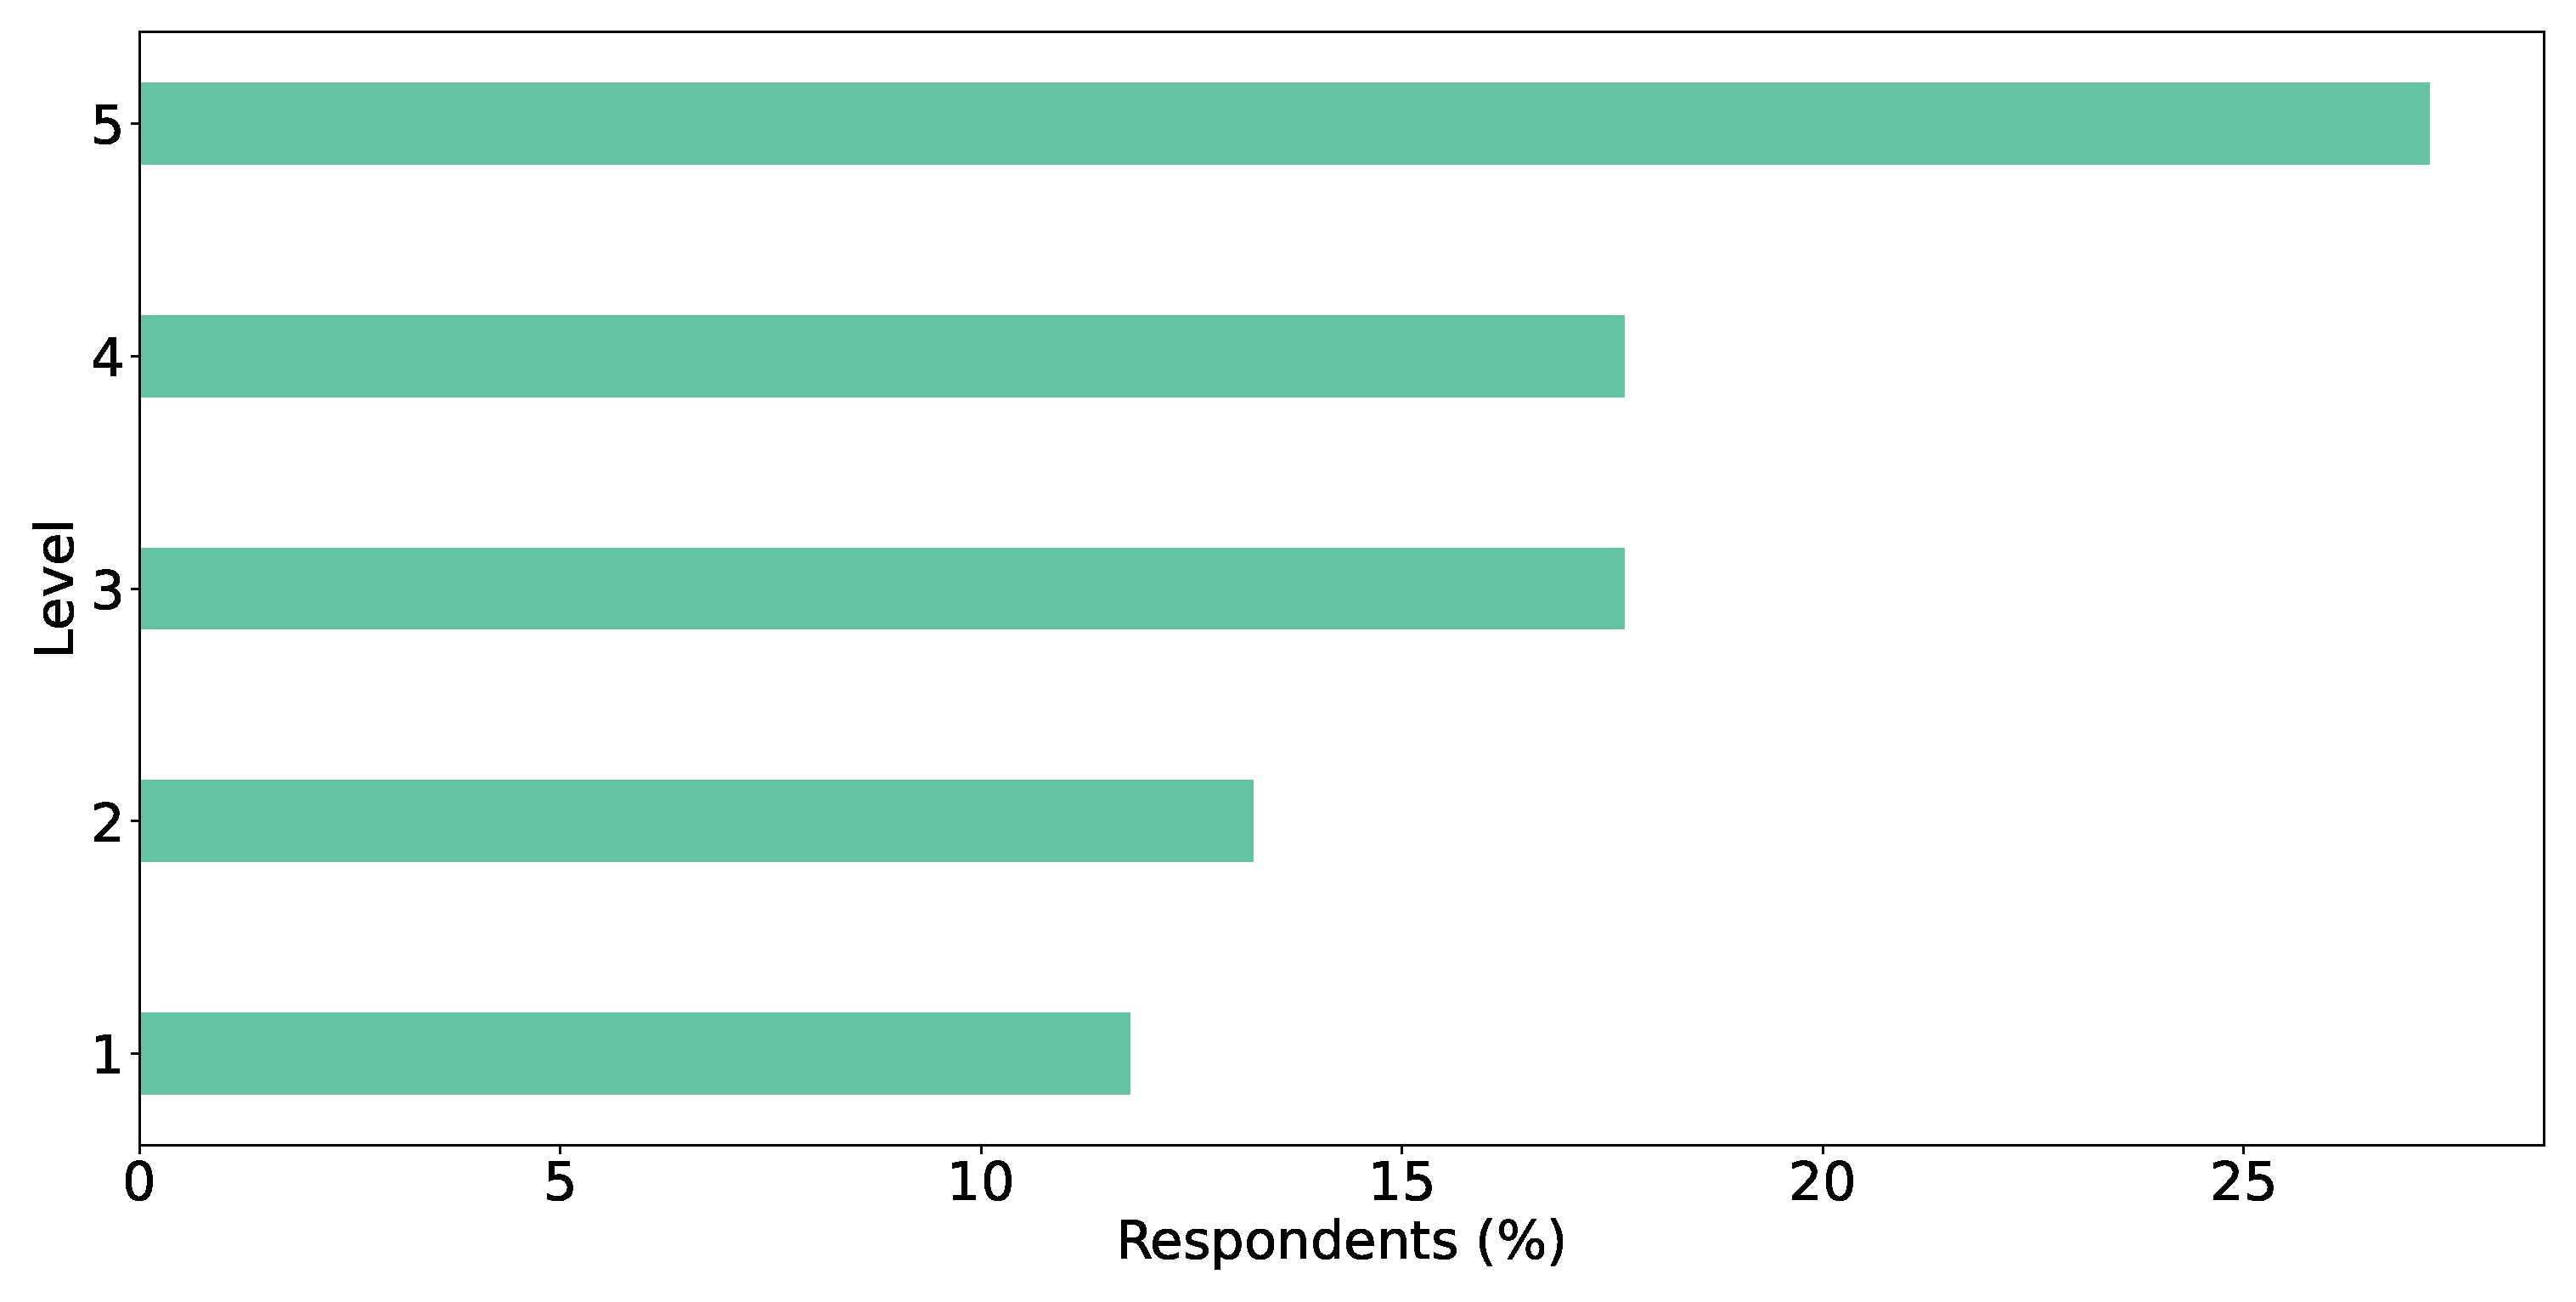
\includegraphics[width=0.8\textwidth]{Figures/Respondents_autotest_level}
  \caption{Automated Testing Level}
  \label{fig:autoTest}
\end{figure}

\subsubsection{Tools Used in Testing and QA}
Q 16 asked about the tools used in testing and quality assurance. According to \cref{fig:testingTools}, we see that most of the respondents have been used XUnit( eg, JUnit, NUnit) (24\%), selenium(21\%), Jenkins(15\%), others(7\%).
\begin{figure}[]
\centering
  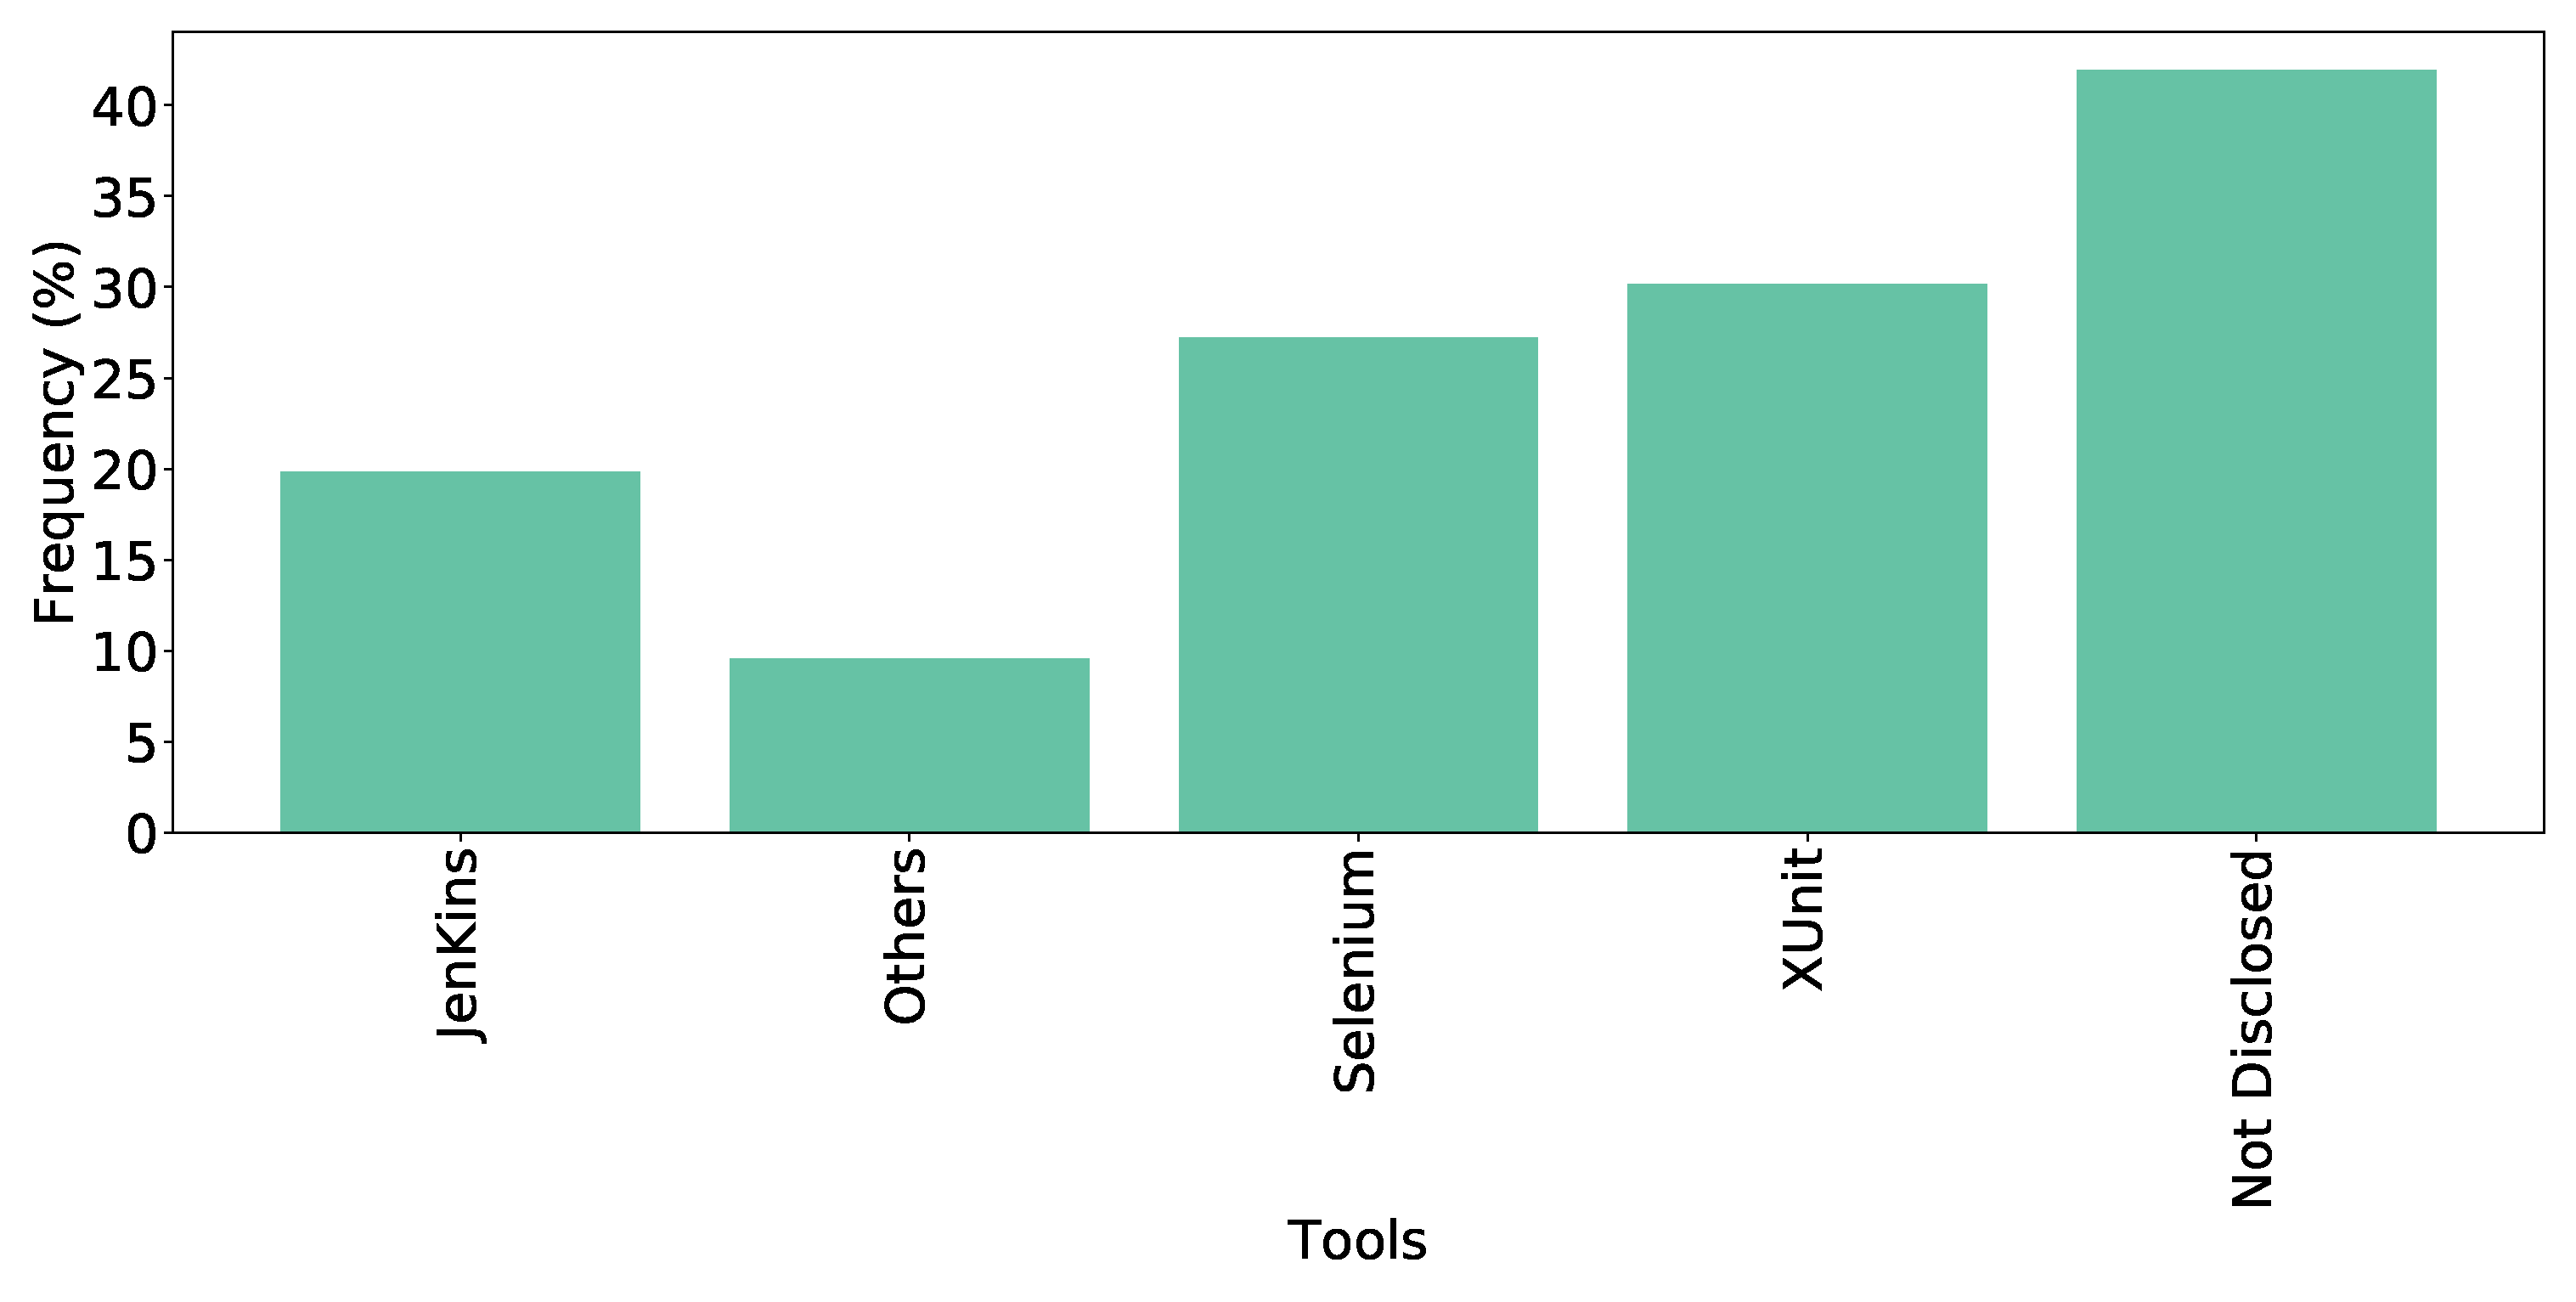
\includegraphics[width=0.8\textwidth]{Figures/Respondents_testing_tools}
  \caption{Testing \& QA Tools}
  \label{fig:testingTools}
\end{figure}

\subsubsection{Deployment Tools}
According to \cref{fig:deployTools}, wee see that most of the respondents use AWS code-deploy(11\%) and JenKins(11\%). The other deployment tools are Bamboo(5\%), teamcity(4\%), octopus(2\%). Respondents voted none (4\%) as they didn’t use any deployment tools.
\begin{figure}[]
\centering
  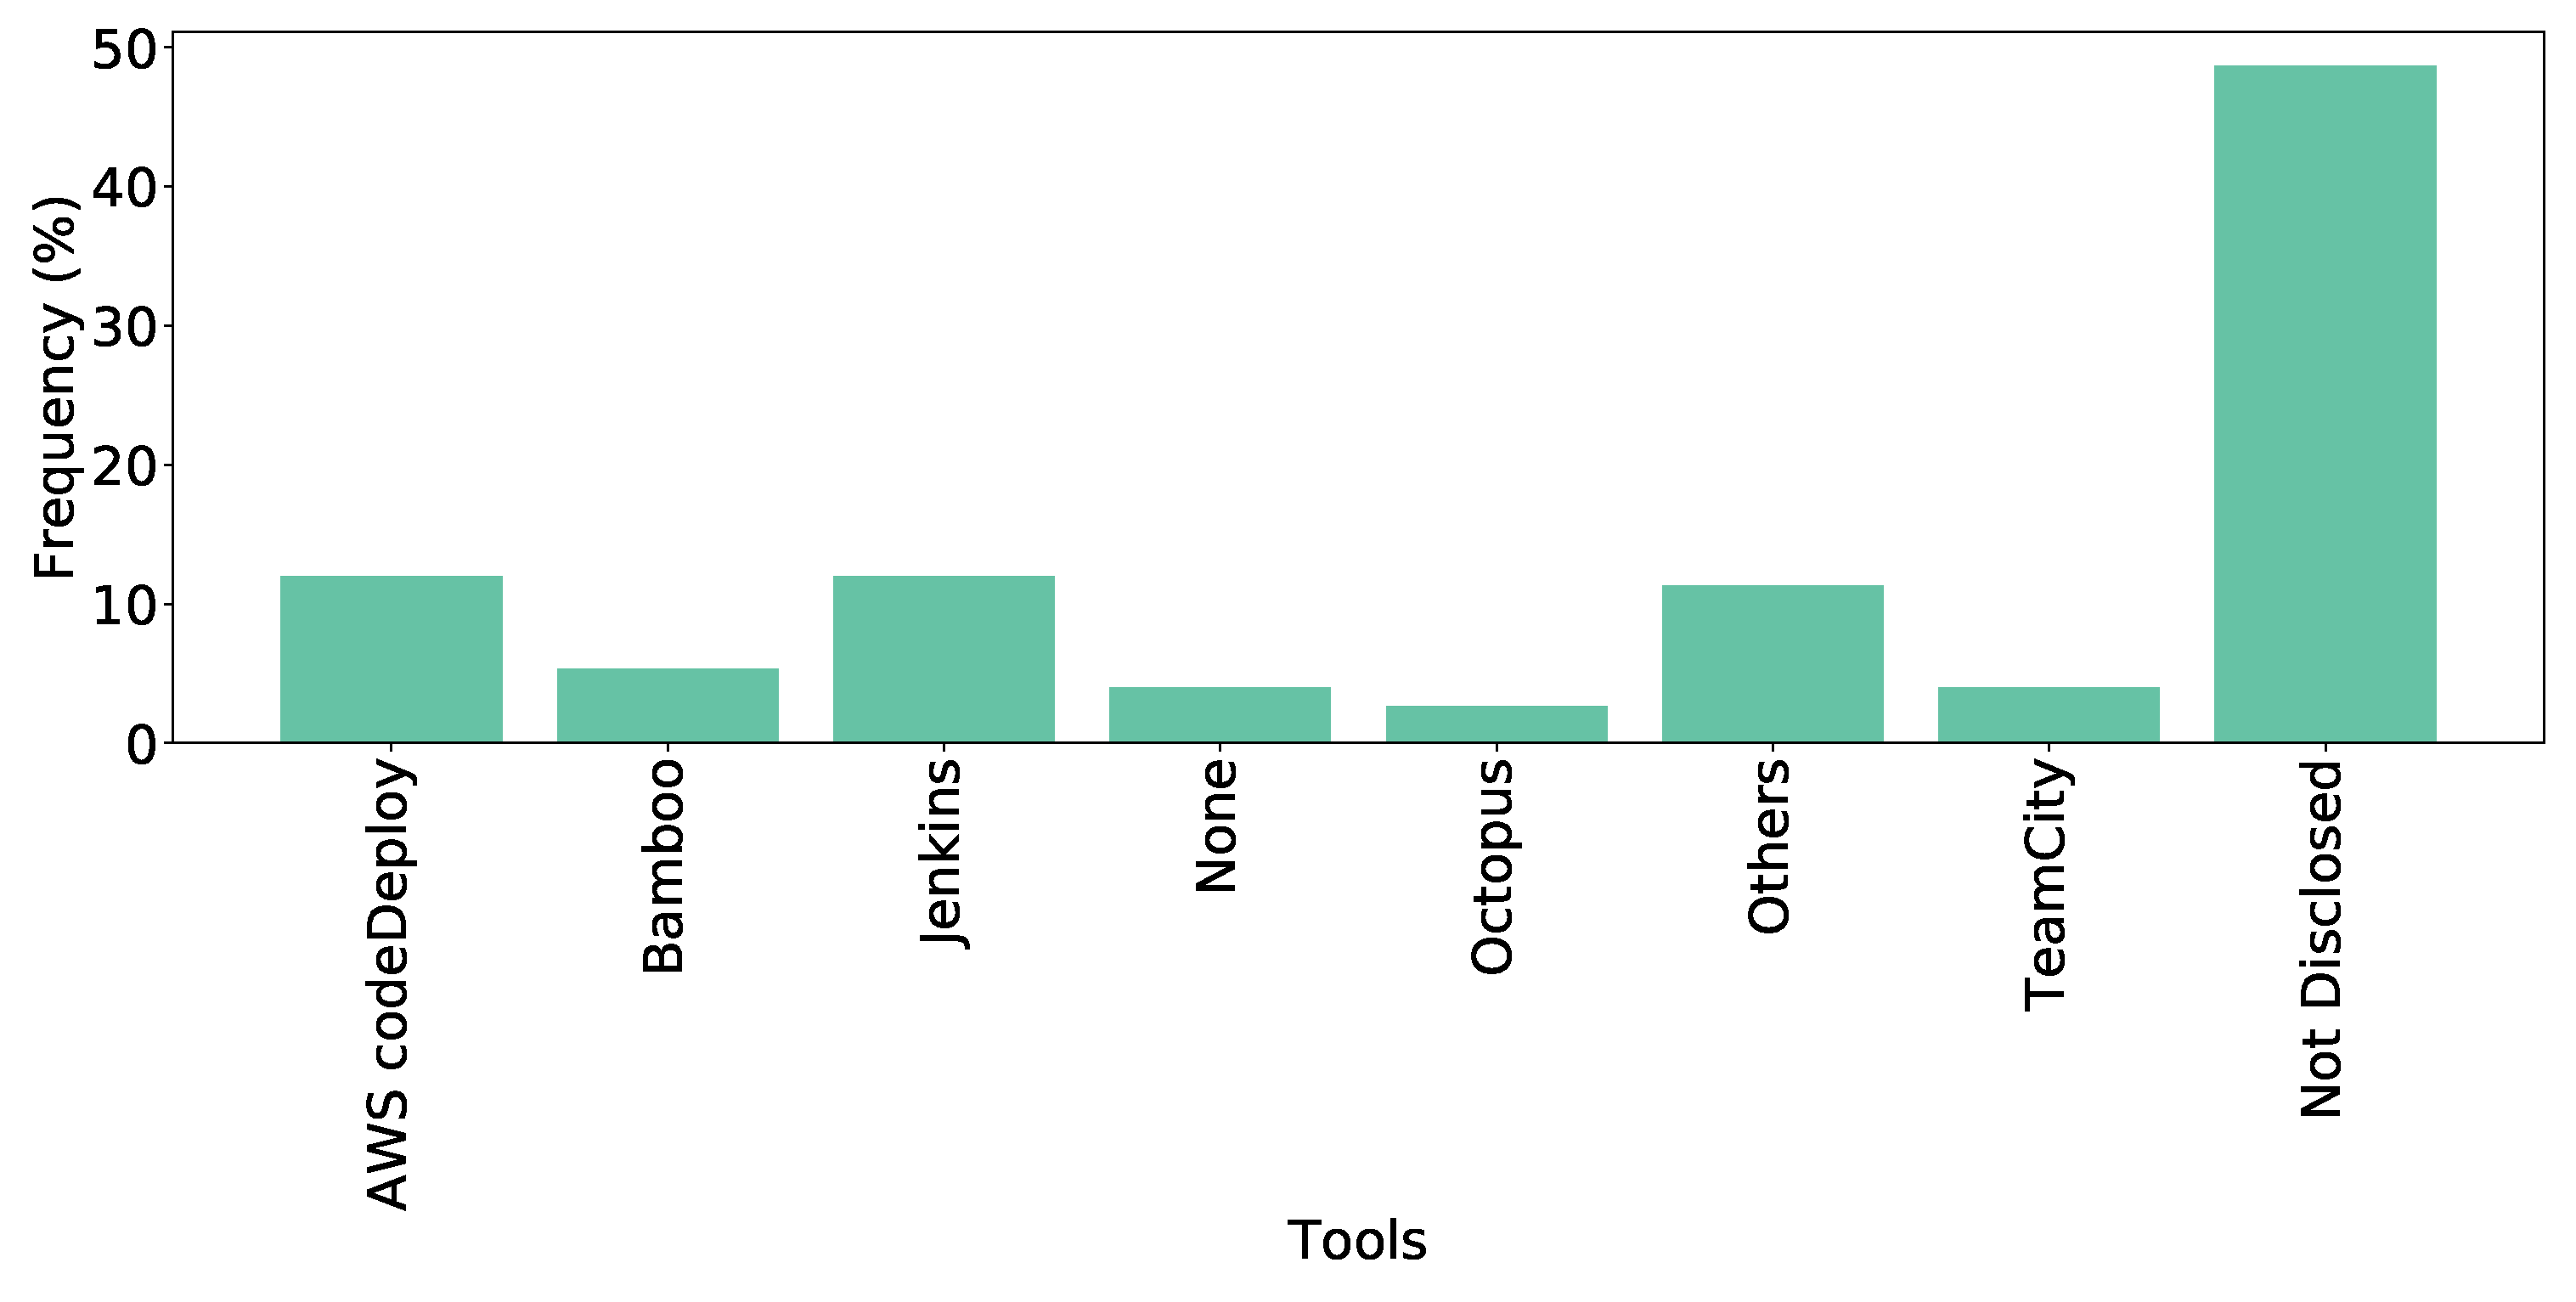
\includegraphics[width=0.8\textwidth]{Figures/Respondents_deployment_tools}
  \caption{Deployment Tools}
  \label{fig:deployTools}
\end{figure}

\subsubsection{Version Control}
Respondents were allowed to select more than one option. As shown in \cref{fig:versionControl}, Git(60\%) and BitBucket(22\%) are mostly-used version control in the software industry. Beside these SVN(4\%), others(3\%) are used.
\begin{figure}[]
\centering
  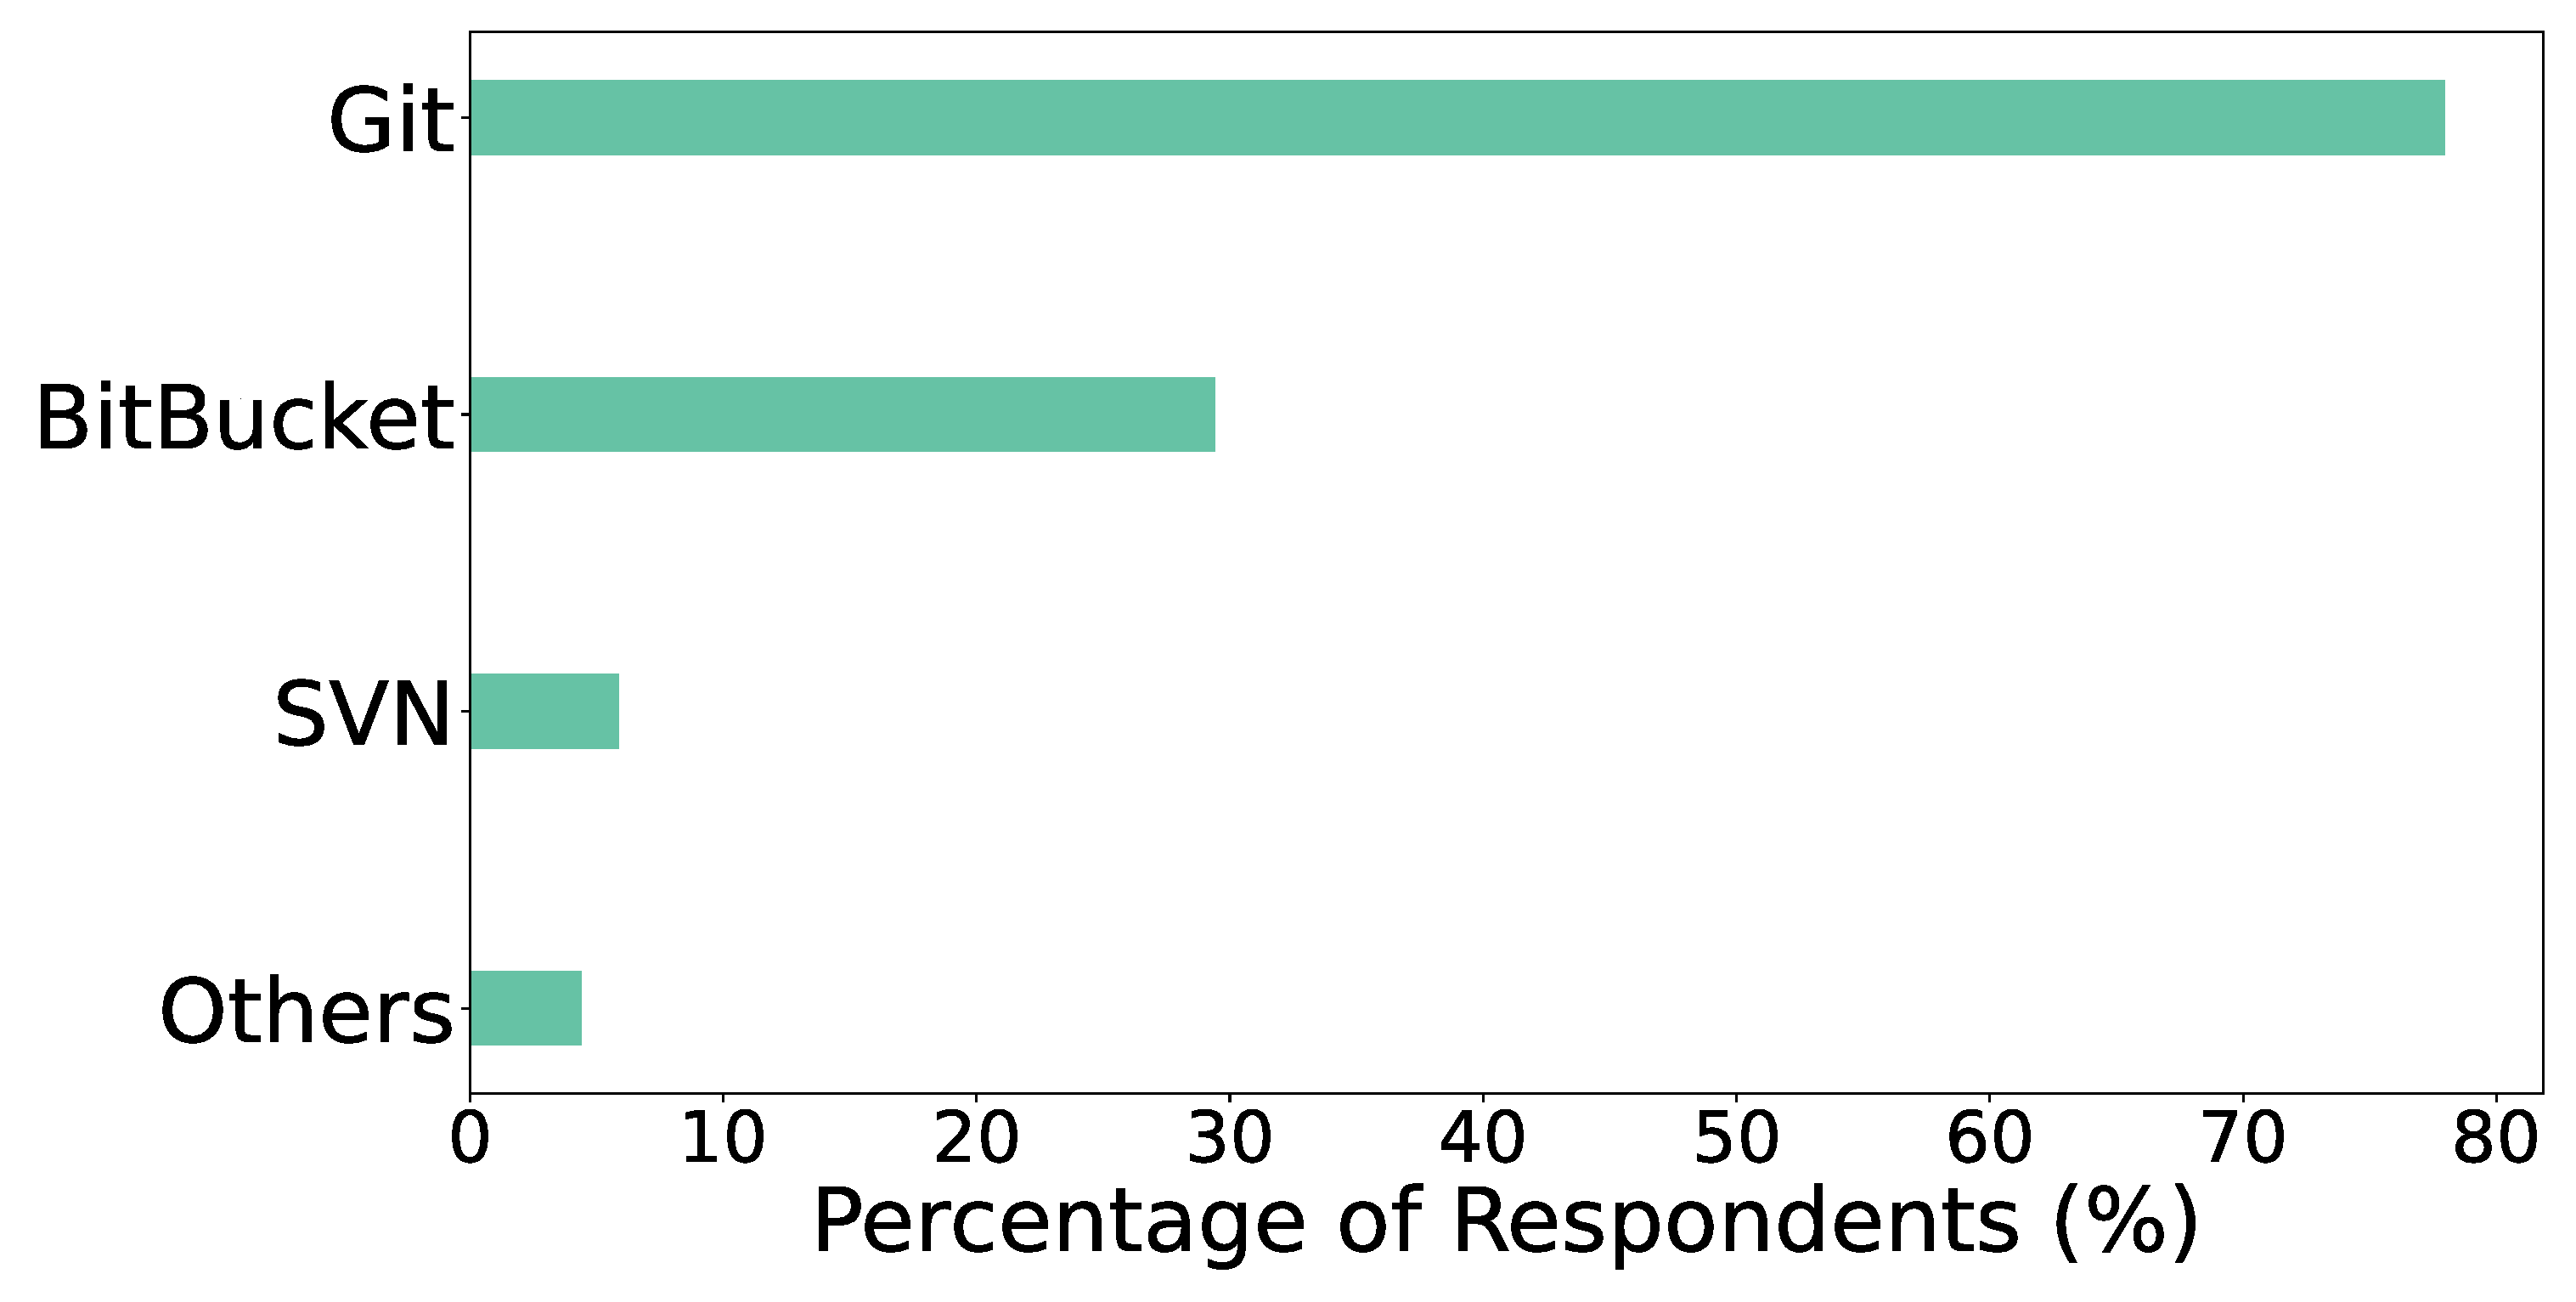
\includegraphics[width=0.8\textwidth]{Figures/Respondents_version_control}
  \caption{Version Control}
  \label{fig:versionControl}
\end{figure}